\subsubsubsubsection{Garage}
\begin{figure}[h]
\centering
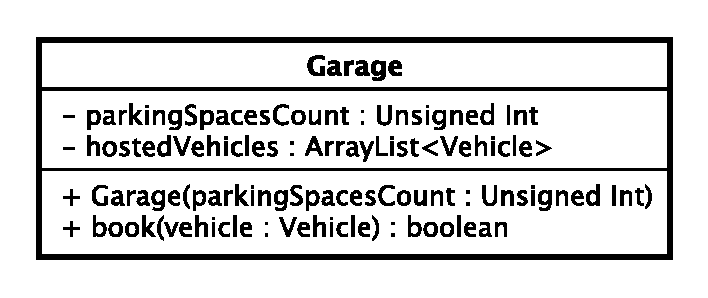
\includegraphics[scale=0.6,keepaspectratio]{images/solution/app/backend/garage.eps}
\caption{\pReactiveComponentStretchDecoration::Garage}
\label{fig:sd-app-garage}
\end{figure}
\FloatBarrier
\begin{itemize}
  \item \textbf{\descr} \\
    It represents a garage which contains parking spaces.
  \item \textbf{\attrs}
  \begin{itemize}
    \item \texttt{parkingSpacesCount : Unsigned Int} \\
The maximum capacity of the garage in number of parking spaces.
    \item \texttt{hostedVehicles : ArrayList<Vehicle>} \\
The collection of vehicles that are currently hosted into the garage.
  \end{itemize}
  \item \textbf{\ops}
  \begin{itemize}
   \item[+] \texttt{\textit{Garage(parkingSpacesCount : Unsigned Int)}} \\
   Creates a garage with a specific capacity.
   \item[+] \texttt{book(vehicle: Vehicle)} \\
   Books a parking space for \texttt{vehicle},
   if there is at least one free parking space.
   \item[+] \texttt{free(vehicle: Vehicle)} \\
   Frees the parking space containing \texttt{vehicle},
   if it is really contained into the garage.
  \end{itemize}
\end{itemize}
